\documentclass[a4paper,12pt]{article} % тип документа

\usepackage[T2A]{fontenc}
\usepackage[utf8]{inputenc}
\usepackage[english,russian]{babel}
\usepackage{amsmath,amsfonts,amssymb,amsthm,mathtools}
\usepackage{wasysym}
\usepackage{graphicx}
\usepackage{wrapfig} \usepackage{float}
\usepackage{amssymb}
\usepackage{ upgreek}
\usepackage{cancel}
\DeclareGraphicsExtensions{.pdf,.png,.jpg}
\addto\captionsrussian{\def\refname{Источники}}

\long\gdef\COMMENT#1{}

\usepackage{xcolor}
\usepackage{hyperref}

\hypersetup{pdfstartview=FitH,  linkcolor=black,urlcolor=blue, colorlinks=true}

\begin{document}
\begin{center}
\bf Лабораторная работа №1 \\
Молодцов Владислав
\end{center}

\section{Задача 1}

Описание циклов представлены в виде комментариев в программе (см. рис. \ref{fig:program_1}).
В данном случае в первой паре циклов, где определяются значения a, никаких зависмостей нет, а в третьей циклов, где происходит вывод значений, используется один и тот же файловый дескриптор, поэтому
их распараллеливание невозможно.
Во второй паре циклов, где происходят сами вычисления, мы имеем loop-carried dependency, поэтому можно параллелить оба цикла, а также переставлять их местами, если очень хочется.

\begin{figure}[h!]
	\center{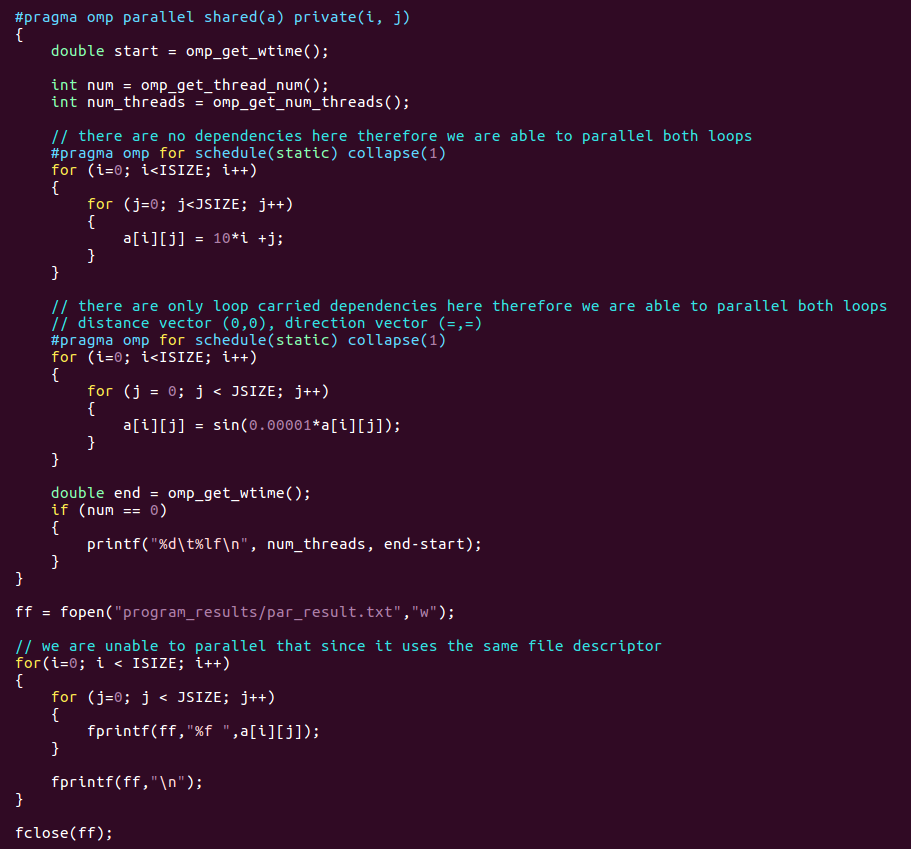
\includegraphics[width=0.9\linewidth] {screenshot_par_1.png}}
	\caption{Параллельная версия программы (файл par\_1.c)}
	\label{fig:program_1}
\end{figure}

\newpage
На рис. \ref{fig:res_1} представлена зависимость времени исполнения первых двух пар циклов от количества исполнителей.
Заметно явное ускорение при увеличении количества исполнителей до 4, а далее
происходит насыщение и начинаются осцилляции, из-за чего прироста не наблюдается. Важно отметить. что эксперименты проводились на 4-х ядерном процессоре с 8-ми потоками, что объясняет такое поведение.

\begin{figure}[h!]
	\center{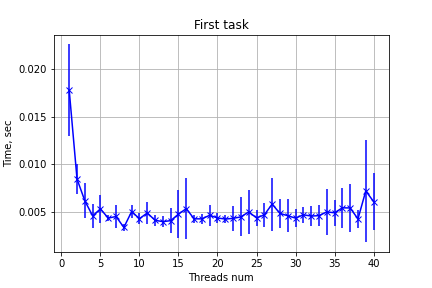
\includegraphics[width=0.8\linewidth] {../results_processing/plot_1.png}}
	\caption{Результаты для задачи 1}
	\label{fig:res_1}
\end{figure}

\section{Задача 2 (1д)}

Описание циклов представлены в виде комментариев в программе (см. рис. \ref{fig:program_2}).
Первая пара циклов та же самая, за исключением того, что теперь там мы производим также резервное копирование массива a в массив b, что пригодится нам в дальнейшем.
Третья пара циклов без изменений, а вот вторая пара циклов
теперь уже имеет loop independent dependencies. Вектор расстояний (-1,6), вектор направлений (>,<), поэтому имеем антизависимость: данные сначала используются, а потом определяются.
Внутренний цикл зависимостей не содержит и по нему можно параллелить без ограничений. А вот по внешнему циклу распараллеливание возможно при условии предварительного резервирования данных.
Отметим, что в данном случае менять циклы местами нельзя: это изменит граф алгоритма.

На рис. \ref{fig:res_2} представлена зависимость времени исполнения первых двух пар циклов от количества исполнителей.
В данном случае также заметно явное ускорение при увеличении количества исполнителей до 4, а далее также
происходит насыщение и начинаются осцилляции, из-за чего прироста не наблюдается, что объясняется количество ядер процессора.

\begin{figure}[h!]
	\center{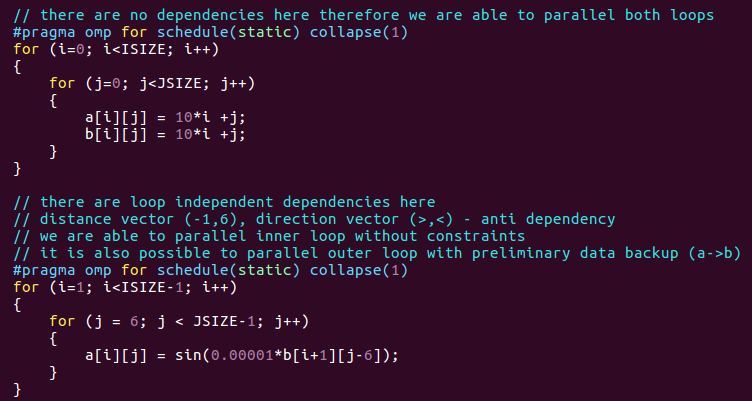
\includegraphics[width=0.9\linewidth] {screenshot_par_2.png}}
	\caption{Параллельная версия программы (файл par\_2.c)}
	\label{fig:program_2}
\end{figure}

\begin{figure}[h!]
	\vspace{-10mm}
	\center{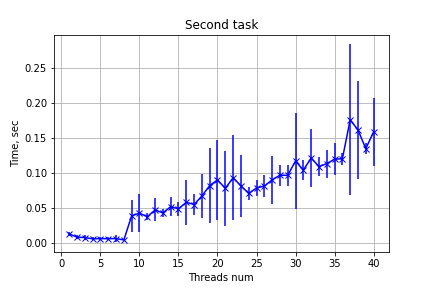
\includegraphics[width=0.8\linewidth] {../results_processing/plot_2.png}}
	\caption{Результаты для задачи 2}
	\label{fig:res_2}
\end{figure}

\section{Задача 3 (2д)}

Описание циклов представлены в виде комментариев в программе (см. рис. \ref{fig:program_3}).
Первая и третья пара циклов как и в задании 1).

Вторая пара циклов теперь имеет loop independent dependencies:
вектор расстояний (8,-3), вектор направлений (<,>), поэтому имеем истинную зависимость: данные сначала определяются, а потом используются.
При это внутренний цикл не содержит зависимостей и может быть распараллелен без ограничений, однако требуется барьерная синхронизация между различными итерациями внешнего цикла.
Распараллелить по внешнему циклу или по двум направлениям не представляется возможным.
Отметим, что в данном случае менять циклы местами также нельзя.

\begin{figure}[h!]
	\center{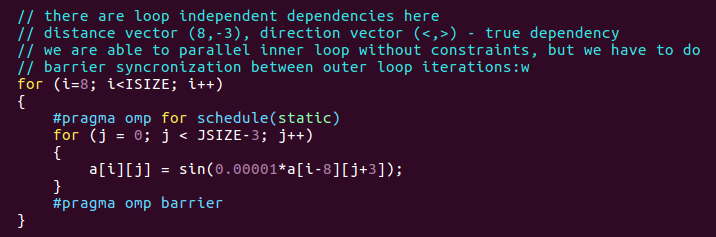
\includegraphics[width=0.9\linewidth] {screenshot_par_3.png}}
	\caption{Параллельная версия программы (файл par\_3.c)}
	\label{fig:program_3}
\end{figure}

\begin{figure}[h!]
	\vspace{-10mm}
	\center{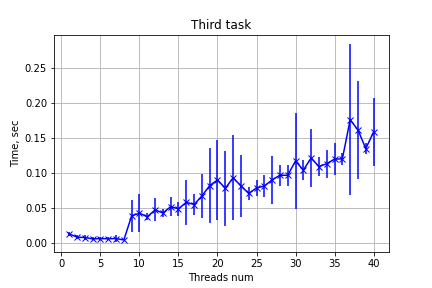
\includegraphics[width=0.8\linewidth] {../results_processing/plot_3.png}}
	\vspace{-5mm}
	\caption{Результаты для задачи 3}
	\label{fig:res_3}
\end{figure}

На рис. \ref{fig:res_2} представлена зависимость времени исполнения первых двух циклов от количества исполнителей.

В данном случае также заметно небольшое ускорение при увеличении количества исполнителей до 4.
Ускорение незначительное, поскольку необходимо использовать большой количество барьеров.
При дальнейшем увеличении числа исполнителей происходит резкое увеличение во времени исполнения программы,
поскольку при большом количестве потоков частые переключения контекста и барьерные синхронизации сильно портят дело.


\end{document}
